\documentclass[a4paper,12pt]{article}
\usepackage{graphicx, float, fancyheadings, a4wide, makeidx, verbatim,avant,helvet}
\usepackage{}
\pagestyle{fancyplain}
\setlength{\parindent}{0pt}
\setlength{\parskip}{6pt}

\newcommand{\param}[1] {\textless{}#1\textgreater{}}

\title{\sf{Datasheet for Infra Red Receiver}}
\lfoot{\tiny{\copyright L.P.Klyne}}

\author{Andy Harris}

\makeindex

\begin{document}

\maketitle

\begin{figure}[H]
\centering

\includegraphics[width=0.4\textwidth]{Images/WebBrickSystems.png}
\end{figure}

\begin{figure}[H]
\centering

\includegraphics[width=0.3\textwidth]{Images/wb_logo.jpg}
\end{figure}


\begin{description}
\item[Feb 2007 Document Version 1.00]
\end{description}

\begin{description}
\item[http:\\www.webbricksystems.com] for company information
\item[http:\\www.webbrick.co.uk] for webbrick information
\end{description}

\pagebreak

\section{Infra Red Emitters}
\index{Infra Red Emitters}

\begin{figure}[H]
\centering
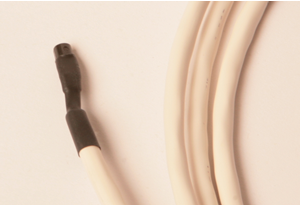
\includegraphics[width=0.4\textwidth]{Images/InfraRedEmitterPic.png}
\end{figure}

\subsection{WebBricks and Infra Red Emitters}

The webbrick can send RC5 infra red commands, this can be the result of a locally configured trigger or remotely 
on request from the WebBrick Gateway:

	\begin{itemize}
	  
	  \item{Cable:} Cat 5E cable is recommended for Infra Red connections. Webbrick Systems supply
	  		Infra Red Emitters with 2M Cat 5E pre-attached.
	  		
	  \item{Bus Length:}  We recommend a maximum bus length of 20M for an emitter.
	  			
	  \item{Unused cores:} We recommend that unused cores are connected to ground.  In particular the brown core
	  			should be connected to ground.
	  			
	\end{itemize}


\subsection{Connections}

The following connections should be made:

\begin{figure}[H]
\centering
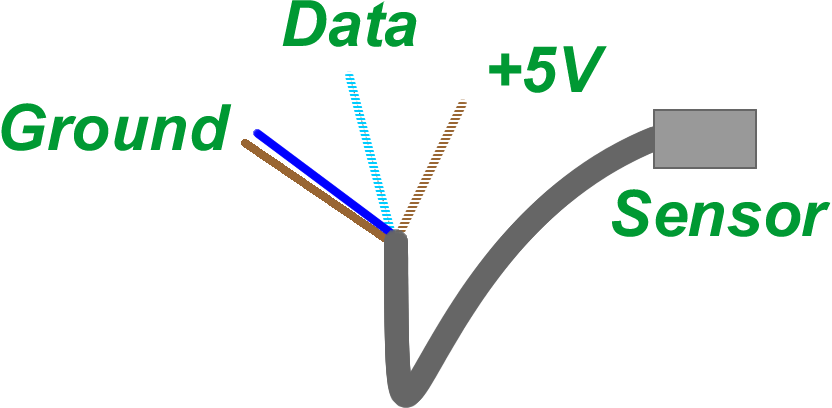
\includegraphics[width=0.6\textwidth]{Images/InfraRedEmitterWiring.png}
\end{figure}

	\begin{itemize}
	  
	  \item{Brown-White:} Connect to digital output 7, highest digital output.
	  		
	  \item{Brown:} Ground.
	  			
	\end{itemize}

If you wish to connect multiple emitters 2 can be connected in parallel to the single output, any more will require buffering.
    
\subsection{Configuration}



\end{document}
